\documentclass[10pt,aspectratio=169]{beamer}

\usetheme{AnnArbor}
\definecolor{offwhite}{RGB}{248,248,245}
\definecolor{darkgreen}{RGB}{0,100,0}
\setbeamercolor{background canvas}{bg=offwhite}
\definecolor{blockbg}{RGB}{235,235,230}
\setbeamercolor{block body}{bg=blockbg, fg=black}
\setbeamercolor{block title}{bg=blockbg!90, fg=black}
\setbeamercolor{alerted text}{fg=red!75!black}
\setbeamertemplate{navigation symbols}{}
\setbeamertemplate{footline}[frame number]
\setbeamersize{text margin left=0.8cm, text margin right=0.8cm}

\usepackage[
  backend=biber,
  style=authoryear,
  citestyle=authoryear-comp,
  maxcitenames=2,
  maxbibnames=99,
  uniquename=false
]{biblatex}
\addbibresource{hiring-bandit.bib}

\usepackage{amsmath,amssymb,bm,booktabs,array}
\usepackage{algorithm}
\usepackage{algorithmic}
\usepackage{graphicx}
\usepackage{tikz}
\usetikzlibrary{arrows.meta,positioning,calc,fit}

\tikzset{
    process/.style={draw, rounded corners, align=center, minimum width=2.25cm, minimum height=9mm, fill=blockbg},
    processarrow/.style={-{Latex[length=2.5mm]}, thick},
    setbox/.style={draw, rounded corners, align=center, minimum width=2.6cm, minimum height=9mm, fill=green!12},
    targetbox/.style={draw, rounded corners, align=center, minimum width=2.6cm, minimum height=9mm, fill=blue!10},
    intermediatebox/.style={draw, rounded corners, align=center, minimum width=2.9cm, minimum height=9mm, fill=orange!18},
    decisionbox/.style={draw, rounded corners, align=center, minimum width=3.1cm, minimum height=11mm, fill=blockbg},
    bigarrow/.style={-{Latex[length=3mm]}, thick}
}

\newcommand{\bE}[1]{{\mathbb{E}\left[#1\right]}}
\newcommand{\OH}{\textsc{Optimistic-Hire}}
\newcommand{\TimeToReplace}{\textsc{TimeToReplace}}
\newcommand{\ChooseTarget}{\textsc{ChooseTarget}}
\newcommand{\ConstructBijection}{\textsc{ConstructBijection}}
\newcommand{\UCB}{\operatorname{UCB}}
\newcommand{\LCB}{\operatorname{LCB}}
\newcommand{\Regret}{\operatorname{Regret}}
\newcommand{\polylog}{\operatorname{polylog}}
\DeclareMathOperator*{\argmax}{arg\,max}

\title{Sequential Hiring of Contingent Workers\\Through Learning-Based Optimization}
\author{Chris Lee}
\institute{University of Michigan}
\date{Prelim Presentation}

\begin{document}

\begin{frame}
  \titlepage
\end{frame}

\begin{frame}{Structure of the Talk}
    \begin{itemize}
        \item Contingent Hiring
        \item Model: Delayed Replacement Bandit
        \item Algorithm Main Ideas
        \item Main Result
        \item Future Work
    \end{itemize}
\end{frame}

\begin{frame}{What are Contingent Workers?}
    \begin{block}{Examples}
    \begin{itemize}
        \item Gig workers
        \item Freelancers
        \item Contractors
        \item Temporary staff from agencies
    \end{itemize}
    \end{block}
    
    \begin{minipage}{0.3\textwidth}
      \centering
      \includegraphics[width=\linewidth]{presentation-images/upwork.png}
    \end{minipage}\hfill
    \begin{minipage}{0.3\textwidth}
      \centering
      \includegraphics[width=\linewidth]{presentation-images/fiverr.png}
    \end{minipage}\hfill
    \begin{minipage}{0.3\textwidth}
      \centering
      \includegraphics[width=\linewidth]{presentation-images/instawork.png}
    \end{minipage}
\end{frame}

\begin{frame}[t]{Contingent Work Is Increasingly Prominent}
\begin{itemize}
    \item Contingent, gig, and freelance work are a visible and important part of modern labor markets \footfullcite{wood2019good,wu2024gig}.
    \item Firms increasingly use these arrangements to\footfullcite{dong2020managing,lobel2024frontiers}:
    \begin{itemize}
        \item manage fluctuating demand
        \item maintain operational flexibility
        \item accesses skills not available in-house
\end{itemize}
    
\end{itemize}
\end{frame}

\begin{frame}{Example: Pickers in a Fulfillment Center}
\begin{columns}[T,onlytextwidth]
    \begin{column}{0.6\textwidth}
        \begin{block}{The Role}
        \begin{itemize}
            \item Locate packages on the inventory shelves
            \item Scan with handheld scanner
            \item Place in totes to be sent to packaging
        \end{itemize}
        \end{block}
        \begin{block}{The Firms Perspective}
        \begin{itemize}
            \item Firms employs \(m\) pickers
            \item Firm \alert{track performance measures} such as time taken to locate each package \parencite{Vincent2015}
            \item Hiring and firing workers is \alert{costly}
            \item New workers must do one shift of unproductive on-boarding so are \alert{not available immediately}
        \end{itemize}
        \end{block}
    \end{column}

    \begin{column}{0.40\textwidth}
        \centering
        \includegraphics[width=\linewidth, height=0.6\textheight, keepaspectratio]{presentation-images/picker.png}
    \end{column}
\end{columns}


\end{frame}

\begin{frame}{Unique Aspects of Contingent Work}
    \begin{block}{Features}
    \begin{itemize}
        \item No long-term commitment
        \item Relatively inexpensive
        \item Often granular worker-level performance data
    \end{itemize}
    \end{block}

    \begin{block}{Challenges}
    \begin{itemize}
        \item Variable worker quality, so staffing choices matter operationally
        \item Often unreliable pre-hire information about worker quality (e.g. rating manipulation on platforms)
    \end{itemize}
    \end{block}

    \begin{alertblock}{Operational Challenge}
        How can firms use performance data and staffing flexibility to improve worker selection?
    \end{alertblock}
    
\end{frame}

\begin{frame}{Existing Hiring Practices}
\begin{columns}[T]
    \begin{column}{0.38\textwidth}
    \begin{itemize}
      \item Resumes
      \item Interviews
      \item Standardized Assessments
      \item Job Trials
    \end{itemize}
    \end{column}

    \begin{column}{0.62\textwidth}
        \begin{minipage}{0.45\textwidth}
          \centering
          \includegraphics[width=\linewidth]{presentation-images/resume.png}
        \end{minipage}\hfill
        \begin{minipage}{0.45\textwidth}
          \centering
          \includegraphics[width=\linewidth]{presentation-images/interview.png}
        \end{minipage}
    
        \vspace{0.5em} 
    
        \begin{minipage}{0.45\textwidth}
          \includegraphics[width=\linewidth]{presentation-images/standardized-assessment.png}
        \end{minipage}
        \hfill
        \begin{minipage}{0.45\textwidth}
          \includegraphics[width=\linewidth]{presentation-images/job-trial.png}
        \end{minipage}
    \end{column}
    \end{columns}
\end{frame}

\begin{frame}{Classic Hiring Practices: Weaknesses}
\begin{itemize}
      \item Resumes  -- Very little \alert{predictive power} \footfullcite{risavy2022resumes}
      \item Interviews
      \begin{itemize}
          \item Unstructured: Modest predictive power but highly susceptible to interviewer \alert{bias} \footfullcite{bohnet2016take}
          \item Structured: Better predictive power, but requires \alert{time}, \alert{expertise}, and \alert{administrative resources} so are often not implemented \footfullcite{roulin2019conducting}
      \end{itemize}
      \item Standardized Assessments -- \alert{expensive} and \alert{difficult} to administer, most firms do not use. \footfullcite{neumann2021implementing}
      \item Job Trials -- In some occupations previous \textbf{on-the-job performance is the best predictor of future performance.} \footfullcite{gordon2006identifying}
    \end{itemize}
\end{frame}

\begin{frame}{Do Classic Hiring Practices Fit Contingent Work?}
    \begin{block}{}
    \begin{itemize}
        \item Relatively inexpensive
        \item Generally unreliable information about quality
        \item No long-term commitment
    \end{itemize}
    \end{block}
    \begin{center}
    \emph{Extensive screening does not make sense.}
    \end{center}
    
    \begin{block}{}
    \begin{itemize}
        \item Repeated interactions
        \item Often have granular performance data \parencite{Vincent2015}
    \end{itemize}
    \end{block}
    \begin{center}
    \emph{We have the ingredients for (statistical) learning.}
    \end{center}

    \begin{alertblock}{Main Idea: Sequential Learning}
        Use worker on-the-job performance to guide future hiring decisions.
    \end{alertblock}
\end{frame}

\begin{frame}{Contingent Hiring as a Sequential Learning Problem}
    \begin{block}{The Firm's Objective}
    \begin{itemize}
        \item Firm operates over periods: \(t=1,\dots, T\)
        \item Firm's objective is to \alert{maximize productivity}
    \end{itemize} 
    \end{block}

    \begin{block}{Worker Productivity}
    \begin{itemize}
        \item Each worker generates random productivity normalized to be in \([0,1]\)
        \item \emph{(Assumption)} Productivity of worker \(i\) is i.i.d. across periods.
    \end{itemize} 
    \end{block}

    \begin{block}{The Firms Decision}
    \begin{itemize}
        \item Employs \(m\) workers (out of \(k\) possible)
        \item Observes the productivity of each of their employed workers in each period
        \item Can change their workforce by implementing \alert{replacements}.
    \end{itemize} 
    \end{block}
    
\end{frame}

\begin{frame}{Modeling Replacements}
    \begin{block}{Definition}
        \begin{itemize}
            \item A \alert{replacement} is a pair \((i,j)\) where \(i\) is a currently employed worker and \(j\) is a currently unemployed worker.
            \item The set of replacements in period \(t\): \(R_t\)
        \end{itemize}
        
    \end{block}

    \vspace{0.5em}
    \begin{itemize}
        \item Replacements are \alert{costly}
            \begin{itemize}
                \item Cost \(c\) paid per replacement
            \end{itemize}
        \item Replacements take time to complete, we call this time the \alert{delay} 
        \begin{itemize}
            \item Replacements \(i,j\) initiated at time \(t\) has random delay: \(\omega_{i,j}^{(t)}\in \mathbb{N}_{\geq 0}\)
            \item \emph{(Assumption)} Delay has bounded mean: \(\bE{\omega_{i,j}^{(t)}}\leq \bar{\omega}<\infty\)
        \end{itemize}
    \end{itemize}
\end{frame}

\begin{frame}{Objective}
\begin{block}{Oracle benchmark}
Let \(A^*\) be the set of the \(m\) best workers in expectation, and let \(\mu(A)=\sum_{i\in A}\mu_i\).
\end{block}

\begin{block}{Objective}
\[
\Regret(T)=\sum_{t=1}^T \bE{\mu(A^*)-\mu(A_t)+c|R_t|}.
\]
\end{block}

\begin{itemize}
    \item \(\mu(A^*)-\mu(A_t)\) captures losses in productivity due to employing a suboptimal workforce.
    \item \(c|R_t|\) captures replacement costs.
    \item Maximize productivity = Minimize regret
\end{itemize}
\end{frame}


% \begin{frame}{Model}
%     \begin{block}{State}
%     \begin{itemize}
%         \item Active workforce \(A_t \subseteq [k]\), \(|A_t|=m\)
%     \end{itemize}
%     \end{block}
    
%     \vspace{0.4em}
    
%     \begin{block}{Action}
%     \begin{itemize}
%         \item Choose a \alert{target workforce}: \(U_t \in \Theta\)
%         \item Initiate replacements: \(R_t:A_t \setminus U_t \to U_t \setminus A_t \)
%         \item Pay cost: \(c|R_t|\)
%     \end{itemize}
%     \end{block}
    
%     \vspace{0.4em}
    
%     \begin{block}{Dynamics}
%     \begin{itemize}
%         \item Each replacement \(i \to j\) completes after a delay \(\omega\) with \(\mathbb{E}\omega\leq \omega_{\max}\)
%         \item Each replacement incurs cost \(c\)
%         \item The active set evolves gradually as replacements complete
%     \end{itemize}
%     \end{block}
% \end{frame}

\begin{frame}{Decision and Information Order Within a Period}
\begin{center}
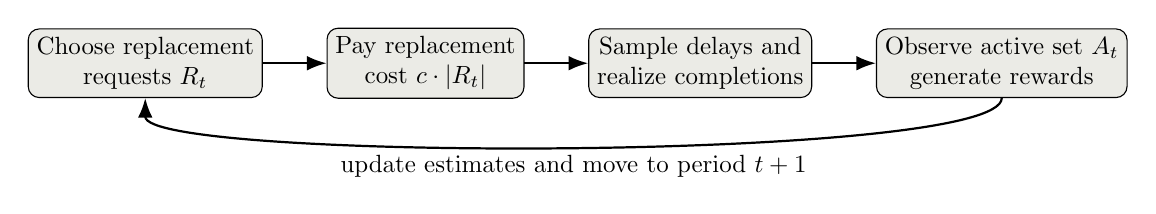
\begin{tikzpicture}[node distance=9mm, transform shape, scale=0.9]
    \node[process] (req) {Choose replacement\\requests \(R_t\)};
    \node[process, right=of req] (cost) {Pay replacement\\cost \(c\cdot |R_t|\)};
    \node[process, right=of cost] (delay) {Sample delays and\\realize completions};
    \node[process, right=of delay] (rew) {Observe active set \(A_t\)\\generate rewards};

    \draw[processarrow] (req) -- (cost);
    \draw[processarrow] (cost) -- (delay);
    \draw[processarrow] (delay) -- (rew);
    \draw[processarrow] (rew.south) .. controls +(0,-0.9) and +(0,-0.9) .. node[midway, below] {update estimates and move to period \(t+1\)} (req.south);
\end{tikzpicture}
\end{center}

\vspace{0.4em}
\begin{block}{Key points}
\begin{itemize}
    \item The firm acts before period-\(t\) rewards are generated
    \item Firm observes rewards \emph{and} the workforce that generated the reward
\end{itemize}
\end{block}
\end{frame}

\begin{frame}[t]{Example}
\begin{columns}[T,onlytextwidth]
    \begin{column}{0.48\textwidth}
        \begin{block}{Suppose the manager currently has}
        \[
            \{1,2,5\}
        \]
        and wants to end up with
        \[
            \{3,4,5\}.
        \]
        The requests are \((1\to 3)\) and \((2\to 4)\).
        \end{block}

        \begin{alertblock}{What actually happens}
        If \((1\to 3)\) completes first, the next productive workforce is \(\{2,3,5\}\), not the target workforce \(\{3,4,5\}\).
        \end{alertblock}
    \end{column}

    \begin{column}{0.48\textwidth}
        \begin{center}
        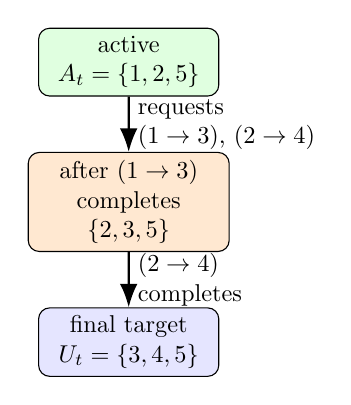
\begin{tikzpicture}[node distance=8mm, transform shape, scale=0.88]
            \node[setbox] (active) {active\\\(A_t=\{1,2,5\}\)};
            \node[intermediatebox, below=of active] (mid) {after \((1\to 3)\)\\completes\\\(\{2,3,5\}\)};
            \node[targetbox, below=of mid] (target) {final target\\\(U_t=\{3,4,5\}\)};

            \draw[bigarrow] (active) -- node[right, align=left] {requests\\\((1\to 3)\), \((2\to 4)\)} (mid);
            \draw[bigarrow] (mid) -- node[right, align=left] {\((2\to 4)\)\\completes} (target);
        \end{tikzpicture}
        \end{center}
    \end{column}
\end{columns}
\end{frame}

\begin{frame}{Related Work}
    \begin{block}{Workforce Management}
    \begin{itemize}
        \item \textbf{Secretary Problems:} permanent decisions and worker productivity immediately available \parencite{dynkin1963optimal, ferguson1989who}
        \item \textbf{Balancing Contingent and Full-Time Workers:} changing the action incurs am additional cost \parencite{king2016dynamic, dong2020managing, berenguer2024managing, lobel2024frontiers}
        \item \textbf{When to Hire/Fire Full-Time Workers:} Worker development and learning over time, modeling human-capital accumulation with Bayesian updating of productivity for full time employees \parencite{arlotto2014optimal}
    \end{itemize}
    \end{block}

    \begin{alertblock}{Gap}
        Do not study how to hire contingent workers with \alert{unknown productivity}.
    \end{alertblock}
\end{frame}

\begin{frame}{Related Work}
    \begin{block}{Multi-Armed Bandits}
    \begin{itemize}
        \item \textbf{Combinatorial semi-bandits:} choose subsets and learn from arm-level feedback \parencite{kveton2014matroid,kveton2015tight}
        \item \textbf{Bandits with switching costs:} changing the action incurs am additional cost \parencite{agrawal1990switching}
        \item \textbf{Bandits with delayed feedback:} observations arrive late, but actions still take effect immediately \parencite{joulani2013online}
        \item \textbf{Blocking bandits:} past actions affect availability through a different mechanism \parencite{basu2019blocking,atsidakou2021combinatorial}
    \end{itemize}
    \end{block}

    \begin{alertblock}{Gap}
        Do not study sequential learning with \alert{action delays}.
    \end{alertblock}
\end{frame}

\begin{frame}
\centering
\vfill
{\LARGE Questions about the Model?}

\vspace{2em}
\centering
\emph{Next, the algorithm...}
\end{frame}

\begin{frame}[t]{Two Main Design Decisions}
\begin{columns}[t]
    \begin{column}{0.48\textwidth}
        \centering
        \textbf{When \& How Often To Replace}
        \vspace{0.5em}
        \raggedright
        \begin{itemize}
            \item Frequent: 
            \begin{itemize}
                \item \textcolor{red}{higher costs} from replacements
                \item \textcolor{darkgreen}{increased flexibility} to find the best workers
            \end{itemize}
            \item Infrequent: 
            \begin{itemize}
                \item \textcolor{darkgreen}{lower cost} from replacements
                \item \textcolor{red}{less flexibility} to find the best workers
            \end{itemize}
            \item Pending replacements: 
                \begin{itemize}
                    \item Can cause replacements to contradict
                    \item Ex. \((i,n)\) and \((j,n)\). If \((i,n)\) completes first, \(j\) is replacing an unemployed worker
                \end{itemize}
        \end{itemize}
    \end{column}

    \begin{column}{0.48\textwidth}
        \centering
        \textbf{Who To Employ}

        \vspace{0.5em}
        \raggedright
        \begin{itemize}
            \item Best performers
            \begin{itemize}
                \item \textcolor{darkgreen}{Better} returns from known workers
                \item \textcolor{red}{Slower} learning
            \end{itemize}
            \item Most uncertain
            \begin{itemize}
                \item \textcolor{red}{Worse} returns from known workers
                \item \textcolor{darkgreen}{Faster} learning
            \end{itemize}
            \item Consider costs
            \begin{itemize}
                \item Is the new (hopefully better) worker worth the replacement cost to employ?
            \end{itemize}
        \end{itemize}
    \end{column}
\end{columns}
\end{frame}

\begin{frame}[t]{Two Main Design Decisions}
\begin{columns}[t]
    \begin{column}{0.48\textwidth}
        \centering
        \textbf{When \& How Often To Replace}
        \vspace{0.5em}
        \raggedright
        \begin{itemize}
            \item Rule \textsc{TimeToReplace}
            \item Frequency:
                \begin{itemize}
                    \item Based on \emph{least observed} worker
                    \item \textcolor{red}{Less} frequent when \textcolor{red}{less} uncertainty
                    \item \textcolor{darkgreen}{More} frequent when \textcolor{darkgreen}{more} uncertainty
                \end{itemize}
            \item Pending replacements: 
                \begin{itemize}
                    \item Wait until none
                \end{itemize}
        \end{itemize}
    \end{column}

    \begin{column}{0.48\textwidth}
        \centering
        \textbf{Who To Employ}

        \vspace{0.5em}
        \raggedright
        \begin{itemize}
            \item Rule \textsc{ChooseTarget}
            \item Use {\bf optimism}
            \begin{itemize}
                \item Favor workers with high upper confidence bounds
            \end{itemize}
            \item Considering costs:
            \begin{itemize}
                \item Only employ when maximum performance gain is plausibly more than the replacement cost
            \end{itemize}
        \end{itemize}
    \end{column}
\end{columns}
\end{frame}

\begin{frame}{High-Level Algorithm Structure}
    \begin{algorithm}[H]
    \small
    \begin{algorithmic}[1]
    \REQUIRE Replacement rule \textsc{TimeToReplace} \qquad \alert{\textbackslash \textbackslash when \& how often to replace}
    \REQUIRE Selection rule \textsc{ChooseTarget} \qquad \qquad  \alert{ \textbackslash \textbackslash who to employ}
    \REQUIRE Pairing rule \textsc{ConstructPairing}
    \FOR{$t = 1,2,\dots,T$}
        \IF{\textsc{TimeToReplace}(\(\mathcal{H}_t\))}
            \STATE Pick intended workerforce using selection rule: $U\gets$ \textsc{ChooseTarget}(\(\mathcal{H}_t\))
            \STATE Construct the replacement: \(R_t\gets \textsc{ConstructPairing}(U, A_t)\)
            \STATE Initiate replacement \(R_t\)
        \ENDIF
        \STATE Update active workforce \(A_t\) with completed replacements
        \STATE Receive reward and observe feedback from \(A_t\)
        \STATE Update statistics \(\mathcal{H}_t\)
    \ENDFOR
    \end{algorithmic}
    \end{algorithm}
\end{frame}


\begin{frame}{Cycle Structure Induced by the Switching Rule}
\begin{center}
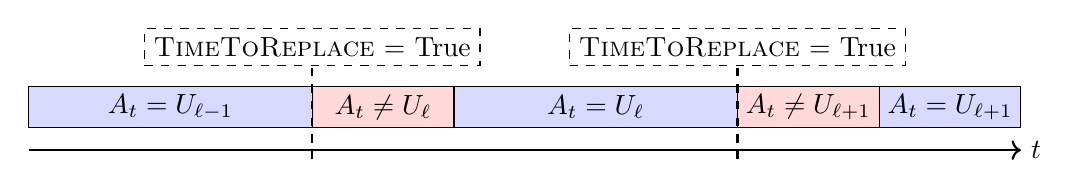
\begin{tikzpicture}[xscale=0.9,yscale=0.95]
    \draw[thick, ->] (0,0) -- (14,0) node[right] {\(t\)};

    \draw[fill=blue!15] (0,0.3) rectangle (4,0.85);
    \node at (2,0.575) {\(A_t=U_{\ell-1}\)};

    \draw[fill=red!15] (4,0.3) rectangle (6,0.85);
    \node at (5,0.575) {\(A_t\neq U_\ell\)};
    \draw[dashed, thick] (4,-0.12) -- (4,1.1);
    \node[draw, dashed, fill=white] at (4,1.38) {\textsc{TimeToReplace} = True};

    \draw[fill=blue!15] (6,0.3) rectangle (10,0.85);
    \node at (8,0.575) {\(A_t=U_\ell\)};

    \draw[fill=red!15] (10,0.3) rectangle (12,0.85);
    \node at (11,0.575) {\(A_t\neq U_{\ell+1}\)};
    \draw[dashed, thick] (10,-0.12) -- (10,1.1);
    \node[draw, dashed, fill=white] at (10,1.38) {\textsc{TimeToReplace} = True};

    \draw[fill=blue!15] (12,0.3) rectangle (14,0.85);
    \node at (13,0.575) {\(A_t=U_{\ell+1}\)};
\end{tikzpicture}
\end{center}

\vspace{0.6em}
Algorithm operates in {\bf cycles} (indexed here by \(\ell\)):
\begin{enumerate}
    \item Select target workforce \(U_{\ell}\) and request replacements to realize new target
    \item \textcolor{red}{Transition phase} (red) 
        \begin{itemize}
            \item Requested replacements are still completing
        \end{itemize}
    \item \textcolor{blue}{Stable phase} (blue) 
    \begin{itemize}
        \item Employed workers are \(U_\ell\)
        \item Insufficient data collected \(U_\ell\)
    \end{itemize}
    \item Conditions needed to initiate new replacement met:
        \begin{itemize}
            \item Indicated by ``\textsc{TimeToReplace}\(=\)True"
            \item Start new {\bf cycle}
        \end{itemize}
\end{enumerate}

\end{frame}

\begin{frame}[t]{Instance-Independent Rate}
\begin{block}{Lower bound}
Any algorithm satisfies
\[
\Regret(T)=\Omega\!\left(\sqrt{mkT}\right)
\]
in the leading dependence on \(T\).
\end{block}

\begin{block}{Upper bound for \OH\ (our proposed algorithm)}
\[
\Regret(T)=\tilde O\!\left(\sqrt{mkT}\right)
\]
up to logarithmic and lower-order friction terms.
\end{block}
\end{frame}

\begin{frame}[t]{Instance-Dependent Rate}
\begin{columns}[T,onlytextwidth]
    \begin{column}{0.48\textwidth}
        \begin{block}{Lower bound}
        In the equal-gap setting, any consistent algorithm satisfies the classical lower-bound form
        \[
            \lim_{T\to \infty}\frac{\Regret(T)}{\log T}=\Omega\!\left(\frac{k-m}{\Delta}\right).
        \]
        \end{block}
    \end{column}

    \begin{column}{0.48\textwidth}
        \begin{block}{Upper bound for \OH}
        In the equal gap setting,
        \[
            \lim_{T\to \infty}\frac{\Regret(T)}{\log T}=
            O\!\left(\frac{k-m}{\Delta}\right)
        \]
        \end{block}
    \end{column}
\end{columns}

\vspace{0.6em}
Delayed and costly replacements preserve the classical leading-order \(\log T / \Delta\) behavior in the instance-dependent regime as well.
\end{frame}


\begin{frame}{Numerical Study: Design}

    \begin{block}{Calibration}
    \begin{itemize}
        \item Inspired by the fulfillment-center example
        \item \(k=150\), \(m=100\) in the main setting
        \item Hourly periods, horizon up to \(5\) years
        \item Delay/cost benchmark: \(\omega_{\max}=8\), \(c=8\) corresponding to a paid, unproductive training shift
        \item Worker means drawn uniformly on \([0.3,0.7]\)
    \end{itemize}
    \end{block}

    \begin{block}{Comparators}
    \begin{itemize}
        \item Delayed-action adaptations of algorithms from the literature \textsc{AgrawalHedgeTezeketzis} \parencite{agrawal1990switching} and \textsc{OMM} \parencite{kveton2014matroid}
        \item Operational heuristics such as semi-annual review and work-trial policies
    \end{itemize}
    \end{block}
\end{frame}

\begin{frame}[t]{Main Benchmark Result}
\begin{columns}[T,onlytextwidth]
    \begin{column}{0.6\textwidth}
        
\includegraphics[width=\linewidth,height=0.68\textheight,keepaspectratio]{paper-images/benchmark_cum_regret.png}
    \end{column}

    \begin{column}{0.4\textwidth}
        \begin{block}{Key Points}
        \begin{itemize}
            \item Lower = Better
            \item Our proposed algorithm is the \textcolor{blue}{blue} line.
            \item Proposed algorithm has the \alert{lowest regret} over horizon
            \item Proposed algorithm exhibits \alert{lower variance} than other policies
        \end{itemize}
        \end{block}
    \end{column}
\end{columns}
\end{frame}


\begin{frame}{Ablations: What Drives the Gains?}
    \small
    \begin{center}
    \begin{tabular}{lrr}
    \toprule
    Variant & 12-month regret & 5-year regret \\
    \midrule
    \OH & \(6{,}462\) & \(11{,}621\) \\
    OH without adaptive switching schedule & \(7{,}785\) & \(16{,}711\) \\
    OH without cost aware selection & \(6{,}765\) & \(12{,}161\) \\
    \bottomrule
    \end{tabular}
\end{center}

\vspace{0.6em}
\begin{block}{Key points}
\begin{itemize}
    \item Largest performance gains come from adaptive switching
    \item Cost-aware selection still valuable, but less imapactful than adaptive switching/.
\end{itemize}
\end{block}
\end{frame}



\begin{frame}{What's next}
    \begin{block}{Model Extensions}
    \begin{itemize}
        \item Contextual information: Worker quality is determined by a set of observable characteristics
        \item Worker-side behavior: quitting and acceptance behavior
    \end{itemize}
    \end{block}

    \begin{block}{Mixed-Noise Combinatorial Semi Bandits}
        \begin{itemize}
            \item Rewards have form: \(\mu_i + \epsilon_i + \eta\) 
            \item \(\epsilon_i\) is stochastic i.i.d. arms \(i\) specific noise.
            \item \(\eta\) is arbitrarily generated noise common among all shared arms.
            \item When can stochastic noise be decoupled from adversarial noise to achieve stochastic regert rates?
        \end{itemize}
    \end{block}
    
\end{frame}

\begin{frame}
    \centering
    \vfill
    {\LARGE Questions?}
    \vfill
\end{frame}

\appendix

\begin{frame}{Appendix: Model Comparison}

\small

\begin{columns}[T,onlytextwidth]
    \begin{column}{0.40\textwidth}
        \begin{block}{Classic CMAB with Switching Costs}
        \begin{itemize}
            \item \textbf{State:} no explicit state beyond last action
            \item \textbf{Control:} choose a set \(A_t \in \Theta\)
            \item \textbf{Played set:} exactly the chosen set \(A_t\)
            \item \textbf{Cost:} \(c\cdot |A_t \setminus A_{t-1}|\)
            \item \textbf{Feedback:} observe \(X_t^{(i)}\) for \(i\in A_t\)
        \end{itemize}
        \end{block}

        \vspace{0.5em}
        \begin{center}
        \[
        \boxed{\text{choose } A_t}
        \;\Longrightarrow\;
        \boxed{\text{play } A_t}
        \]
        \end{center}

        \begin{center}
        \emph{Decision = action executed immediately}
        \end{center}
    \end{column}

    \begin{column}{0.56\textwidth}
        \begin{block}{Delayed Replacement Bandit}
        \begin{itemize}
            \item \textbf{State:} active set \(A_t\), \(|A_t|=m\)
            \item \textbf{Control:} choose replacements
            \[
            R_t:(A_t\setminus U_t)\to (U_t\setminus A_t)
            \]
            for some target set \(U_t\in\Theta\)
            \item \textbf{Played set:} current active set \(A_t\)
            \item \textbf{Cost:} \(c\) per initiated replacement
            \item \textbf{Dynamics:} replacements complete after delays
        \end{itemize}
        \end{block}

        \vspace{-2em}
        \begin{center}
        \[
        \boxed{\text{choose replacements } R_t}
        \;\Longrightarrow\;
        \boxed{\text{active set evolves over time}}
        \]
        \end{center}

        \begin{center}
        \emph{Decision changes the played set only gradually}
        \end{center}
    \end{column}
\end{columns}
\end{frame}

\begin{frame}{Appendix: Deriving a Switching Rule}
    \begin{block}{Effects of Delays}
    \begin{itemize}
        \item \textbf{Fixed (calendar based) switching:}
        \begin{itemize}
            \item Switch every preset number of periods
            \item Delays may cause the policy to collect insufficient data for some workers during the preset periods.
        \end{itemize}
        \vspace{0.3em}
        \item \textbf{Adaptive (count based) switching:}
        \begin{itemize}
            \item Switch when a prescribed amount of data about the current workforce has been collected.
            \item Can respond to delays by waiting to initiate replacements based on the amount of data actually collected
        \end{itemize}
    \end{itemize}
    \end{block}
    
    \vspace{0.5em}
    
    \begin{alertblock}{Design Principle 2}
        When to initiate replacements should be \emph{adaptive} and able to respond to realized delays.
    \end{alertblock}
\end{frame}

\begin{frame}{Appendix: Single-Play Illustration: A Switching Schedule}
    \begin{block}{Setup}
    \begin{itemize}
        \item Let \(T_i(t)\) be the number of times arm \(i\) has been played
        \item Let \(\gamma\) be a tunable parameter
        \item No delays
    \end{itemize}
    \end{block}
    
    \begin{block}{Switching Rule}
    \begin{itemize}
        \item Suppose arm \(i\) is selected by \textsc{ChooseTarget}(\(\cdot\)) in period \(\ell\)
        \item Define
        \[
            \textsc{TimeToReplace}(t)=\begin{cases}
                \textsc{True}, &\text{if } T_i(t)\geq T_i(\ell)+2\sqrt{\gamma T_i(\ell)} + \gamma\\
                \textsc{False}, &\text{otherwise}
            \end{cases}
        \]
        \item Intuition: Do not initiate new replacements until \(i\) has been played for \(2\sqrt{\gamma T_i(\ell)} + \gamma\) additional periods.
    \end{itemize}
    \end{block}
\end{frame}

\begin{frame}{Appendix: Single-Play Illustration: Number of Switches}
    \begin{block}{Growth of Play Counts}
    Let \(a_n\) be the number of plays of an arm after its \(n\)-th selection. Then
    \[
    a_n = a_{n-1} + 2\sqrt{\gamma a_{n-1}} + \gamma \quad \Rightarrow \quad a_n \approx \gamma n^2.
    \]
    \end{block}
    
    \vspace{0.5em}
    
    \begin{block}{Simple Result}
    \begin{itemize}
        \item (Claim) The most switches occur when we play all arms equally
        \item In this case, each arm can be selected at most \(O\left(\sqrt{T/(\gamma k)}\right)\) times
        \item Therefore,
        \[
        \#\text{ switches} \;\le\; k \cdot \sqrt{\frac{T}{\gamma k}} = \sqrt{\frac{kT}{\gamma}}\in O(\sqrt{kT}).
        \]
    \end{itemize}
    \end{block}
    \begin{center}
    \emph{This bound depends only on the switching schedule, not on} \textsc{ChooseTarget}(\(\cdot\))
    \end{center}
\end{frame}

\begin{frame}{Appendix: From Single-Play to Delayed Multi-Play}
    \begin{block}{What drove the schedule?}
    \begin{itemize}
        \item In single-play, the length of the wait depends on the play count:
        \[
        \text{length} \sim \sqrt{T_i(t)}
        \]
        \item This ensures:
        \begin{itemize}
            \item sufficient data is collected before switching
            \item switching frequency decreases over time
        \end{itemize}
    \end{itemize}
    \end{block}
    
    \vspace{0.5em}
    
    \begin{block}{Delayed Multi-Play Setting}
    \begin{itemize}
        \item Now we select a \emph{set} \(U_\ell\) of workers
        \item Different workers in \(U_\ell\) may have very different play counts
        \item Need to ensure delays do not cause replacements to conflict
    \end{itemize}
    \end{block}
    
    \vspace{0.5em}
    
    \centering
    \emph{How do we map the \(m\) play counts to a switching rule?}
\end{frame}

\begin{frame}{Appendix: Adaptive Switching Rule}
\begin{algorithm}[H]
    \caption{TimeToReplace}
    \begin{algorithmic}[1]
        \REQUIRE Switching parameter \(\gamma>0\)
        \REQUIRE Most recent switch time \(d_\ell\)
        \STATE Compute least-sampled worker:
        \[
            i^- \in \arg\min_{j \in U_\ell} T_j(d_\ell)
        \]
        \STATE Compute threshold:
        \[
            N(\ell)\gets \left\lceil 2\sqrt{\gamma\, T_{i^-}(d_\ell)} + \gamma \right\rceil
        \]
        \IF{\(T_{i^{-}}(t)\geq T_{i^{-}}(d_{\ell}) + N(\ell)\) and \(A_t=U_\ell\)}
            \RETURN True
        \ELSE
            \RETURN False
        \ENDIF
    \end{algorithmic}
\end{algorithm}
\end{frame}

\begin{frame}{Appendix: Selection Rule}
\small
\begin{block}{Confidence bounds}
\[
\UCB_i(t)=\bar{\mu}_i(t)+\sqrt{\frac{\log T}{T_i(t)}},
\qquad
\LCB_i(t)=\bar{\mu}_i(t)-\sqrt{\frac{\log T}{T_i(t)}}.
\]
For a possible replacement \(i\to j\), define \(\delta_{i,j}(t)=\UCB_j(t)-\LCB_i(t)\).
\end{block}

\begin{block}{Appendix: Target-selection problem}
\begin{align*}
    \argmax_U &\quad \sum_{i\in U}\UCB_i(t)\\
\quad\text{subject to}&\quad
\sum_{i\in A_t\setminus U}\delta_{i,\pi^R(i)}(t)\ge c\,\frac{|A_t\setminus U|}{T-t}
\end{align*}
\end{block}

\begin{itemize}
    \item Objective: optimistic choice of the target workforce
    \item Constraint: only request replacements whose upside can plausibly pay back their cost over the remaining horizon
\end{itemize}
\end{frame}

\begin{frame}[t]{Appendix: Pairing Rule}
    \small
    Let \(A^-\) be the workers scheduled to leave the active workforce and \(A^+\) denote those scheduled to enter.
    \begin{block}{Rank-matching construction}
    Order the arms in \(A^-=\{i_1,\dots,i_r\}\) and \(A^+=\{j_1,\dots,j_r\}\) by decreasing LCB
    \[
    \LCB_{i_1}(t)\ge \cdots \ge \LCB_{i_r}(t),
    \qquad
    \LCB_{j_1}(t)\ge \cdots \ge \LCB_{j_r}(t).
    \]
    Define the pairing
    \[
    \pi^R(i_s)=j_s,\qquad s=1,\dots,r,
    \]
    and request
    \[
    R_t=\{(i_s,j_s):s=1,\dots,r\}.
    \]
    \end{block}

    \begin{center}
    \emph{The pairing determines which intermediate workforces arise during the transition.}
    \end{center}
\end{frame}

\begin{frame}[t]{Appendix: Instance-Dependent Guarantee}
\small
\begin{block}{Lower bound}
For Bernoulli instances with gap \(\Delta\), any consistent algorithm satisfies
\[
\liminf_{T\to\infty}\frac{\Regret(T)}{\log T}\ge \Omega\!\left(\frac{k-m}{\Delta}\right).
\]
\end{block}

\begin{block}{Upper bound for \OH}
Under unique best workers,
\[
\Regret(T)
\le
C_1\sum_{j>m}\frac{\log T}{\Delta_{m,j}}
\;+\;
\text{lower-order friction terms}.
\]
\end{block}
\end{frame}

\begin{frame}[t]{Appendix: Computing \ChooseTarget}
\begin{columns}[T,onlytextwidth]
    \begin{column}{0.58\textwidth}
        \begin{block}{Reduction}
        \begin{itemize}
            \item Fix the number \(r\) of replacements
            \item Take the \(r\) inactive workers with the largest UCBs on the entering side
            \item Choose which \(r\) active workers to remove
        \end{itemize}
        \end{block}

        \begin{block}{Implementation}
        The remaining problem is a cardinality-constrained knapsack solved exactly by a frontier-based dynamic program.
        \end{block}
    \end{column}

    \begin{column}{0.38\textwidth}
        
\includegraphics[width=\linewidth]{paper-images/OH_frontier_size.png}

        \vspace{0.4em}
        {\small Benchmark runtime: about \(27\) ms per \ChooseTarget\ call and about \(5\) seconds for a full five-year run.}
    \end{column}
\end{columns}
\end{frame}


\begin{frame}[t]{Appendix: Pairing Results}
\small
\begin{block}{Surrogate transition criterion}
For a pairing \(\pi:A^- \to A^+\) and realized delays \(\omega\),
\[
Z(\pi;\omega)=\sum_{i\in A^-}\Bigl(\omega_{i,\pi(i)}\,\LCB_i+(\omega_{\max}-\omega_{i,\pi(i)})\,\LCB_{\pi(i)}\Bigr).
\]
This is a conservative proxy for worst intermediate-workforce performance during the transition.
\end{block}

\begin{block}{Worst-case bounded delays}
Rank matching minimizes a conservative surrogate notion of transition regret over all feasible bijections.
\end{block}

\begin{block}{i.i.d.\ delays}
\begin{itemize}
    \item All bijections have the same expected worst-case transition reward
    \item Rank matching minimizes the variance of realized transition reward
\end{itemize}
\end{block}
\end{frame}


\begin{frame}{Appendix: Proof Roadmap}
\begin{center}
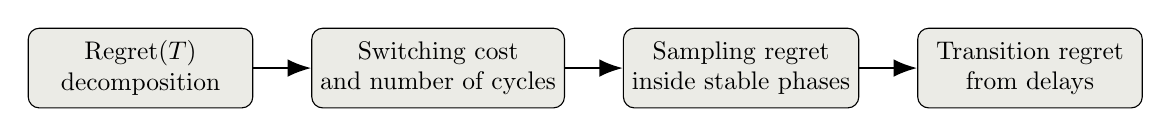
\begin{tikzpicture}[node distance=8mm, transform shape, scale=0.92]
    \node[decisionbox] (decomp) {\(\Regret(T)\)\\decomposition};
    \node[decisionbox, right=of decomp] (switch) {Switching cost\\and number of cycles};
    \node[decisionbox, right=of switch] (block) {Sampling regret\\inside stable phases};
    \node[decisionbox, right=of block] (trans) {Transition regret\\from delays};

    \draw[bigarrow] (decomp) -- (switch);
    \draw[bigarrow] (switch) -- (block);
    \draw[bigarrow] (block) -- (trans);
\end{tikzpicture}
\end{center}

\vspace{0.7em}
\begin{block}{Two key innovations}
\begin{itemize}
    \item A pathwise packing argument for the adaptive switching rule
    \item A sampling-regret decomposition with a delay-induced bookkeeping term that telescopes across cycles
\end{itemize}
\end{block}
\end{frame}

\begin{frame}[t]{Appendix: Proof Idea I: Number of Switches}
\begin{block}{Difficulty}
Block lengths are \emph{endogenous}: they depend on realized play counts, not on a fixed calendar.
\end{block}

\begin{block}{Idea}
Study the most switch-heavy admissible sequence of target workforces. That extremal sequence can be used to produce deterministic bounds on the number of switches.
\end{block}

\begin{alertblock}{Consequence}
The number of switching cycles satisfies
\[
L=O\!\left(\sqrt{\frac{kT}{\gamma}}\right)
\]
up to logarithmic factors.
\end{alertblock}
\end{frame}

\begin{frame}[t]{Appendix: Proof Idea II: Sampling Regret in Block Phases}
\small
\begin{itemize}
    \item In block phases, the active workforce equals the target workforce
    \item For each suboptimal worker, we can decompose regret into the frictionless learning regret and regret due to limiting switches.
    \item Bounding the frictionless learning regret yields the classical \(\log T/\Delta\) term
    \item The regret from limiting switches can be bounded via a telescoping sum to be of lower order.
\end{itemize}

\begin{alertblock}{Key Challenge}
    Delays separate the time of decisions and when rewards are generated, requiring changes to the analysis throughout.
\end{alertblock}
\end{frame}

\begin{frame}[t]{Appendix: Proof Idea III: Sampling Regret in Transition Phases}
\begin{itemize}
    \item During a transition, the active workforce may contain a mix of old and new workers
    \item Each epoch contributes at most \(O(\omega_{\max}m)\) transition regret
    \item Since there is only one transition per switch, the machinery used for bounding the switching cost can be reused to bound the transition regret.
\end{itemize}
\end{frame}
\end{document}
